% !TEX root = ../main.tex
% --+ The parton model +--------------------------------------------------------
\begin{figure}[b!] % NOTE. Figure out source.
    \centering\frame{
    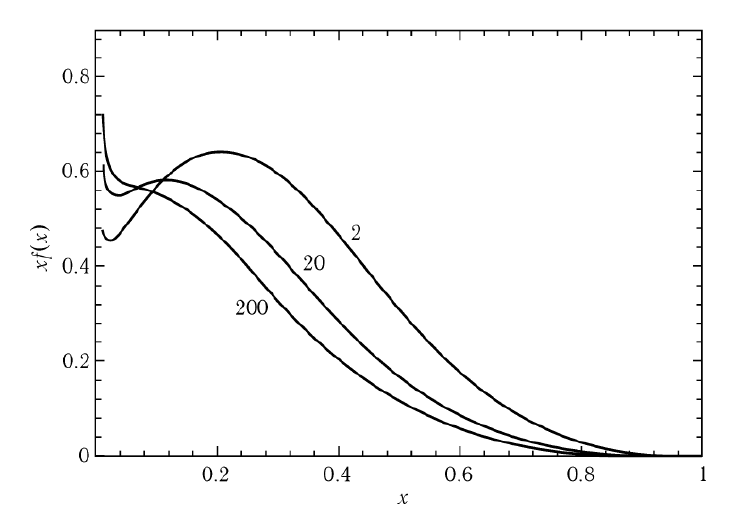
\includegraphics[width=0.8\textwidth]{10physicsmotivation/img/10q2_dependence_u.png}}
    \caption[$Q^2$ dependence of $x$ PDF for the $u$ quark.]{$xf_f(x)$ parton distribution functions for the $u$ quark when $Q = 2$, $Q = 20$, and $Q = 200$ GeV.
    The plots show the parton evolution effect according to the Altarelli-Parisi equations.}
    \label{fig::q2dependenceu}
\end{figure}

In the parton model, the cross section is
\begin{equation}
    \label{eq::parton_model_cross_section}
    \frac{d^2\sigma}{dxdy} \left( e^-p \rightarrow e^-X \right) =
            \left( \sum_f xf_f \left( x, Q^2 \right) Q_f^2 \right)
            \frac{2\pi\alpha s}{Q^4} \left( 1 + \left( 1 - y \right)^2 \right),
\end{equation}
where $s \equiv 2P\cdot k$, $Q_f$ is the charge of the parton $f$, and $x$ and $y$ are the Bjorken variables, defined as
\begin{equation*}
    x \equiv \frac{Q^2}{2P\cdot q}, \hspace{36pt} y \equiv \frac{2 P\cdot q}{s}.
\end{equation*}
In the nucleon's rest frame, $y = q^0/k^0$, and thus it is the energy transferred to the hadron by the incoming electron.

Due to gluon radiation, the PDFs in equation \eqref{eq::parton_model_cross_section} have a weak dependence on $Q^2$.
This leads to Bjorken scaling violation \cite{halzen1991}.
When the structure functions are known for certain values of $Q^2$, they can be evolved to other values using the Dokshitser-Gribox-Lipatov-Altarelli-Parisi (DGLAP) equations \cite{dokshitzer1991}.

Figure \ref{fig::q2dependenceu} shows the predictions of the Altarelli-Parisi equations for the evolution of the PDFs dependence on $Q^2$.
Partons with large $x$ tend to radiate and move to states with lower $x$.
Parallel to this, the radiations produce new partons with low $x$ values.
With an increase in $Q^2$, the parton distributions decrease for large $x$ values, while quickly increasing for low $x$.
At low $Q^2$, the wavelength of the virtual photon is too large to probe the partons, thus probing the proton as a whole.
The validity range for the QCD-extended parton model is not precisely known, but is assumed to be valid for $Q^2 > 1 \text{ GeV}^2$, corresponding to a spatial resolution of about $0.2$ fm.
